\documentclass{article}
\usepackage[utf8]{inputenc}
\usepackage{graphicx}
\usepackage{float}

\title{COL380: Assignment 0}
\author{Sachin 2019CS10722 }
\date{January, 2022}

\begin{document}

\maketitle

\section{Changes Made: }
\subsection{Makefile}
\begin{enumerate}
\item Added flags -g and -pg (required for running of profiliers)
\item Compiled using -fopenmp
\item Added make test command to change variables using command line arguments (for testing)
\item Added make clean command

\end{enumerate}
So run makefile with following optional arguments for testing: \\
\hspace*{1cm} make test r=$<a1>$ d=$<a2>$ n=$<a3>$ t=$<a4>$ x=$<a5>$\\
where, \\
\hspace*{1cm} a1 = range file\\
\hspace*{1cm} a2 = data file\\
\hspace*{1cm} a3 = max data to read\\
\hspace*{1cm} a4 = number of threads\\
\hspace*{1cm} a5 = reps\\

by default, a1 = rfile, a2 = dfile, a3 = 1009072, t = 4, x = 3\\

\subsection{classify.h}
\begin{enumerate}
\item Returned *this in the operator+= function of Ranges class (as pointed out in piazza).
\item Added function \textbf{increaseVal}(unsigned int \textbf{id}, int \textbf{val}) in class Counter, that increase count of id by val.
\end{enumerate}

\pagebreak
\subsection{classify.cpp}
During parallel computation the given code is dividing between multiple threads in following way:- \\
\begin{figure}[H]
    \centering
    \includegraphics[width=8cm]{t1.jpg}
    \caption{Original Code}
\end{figure}

I've changed it in following way:- \\
\begin{figure}[H]
    \centering
    \includegraphics[width=8cm]{t2.jpg}
    \caption{Modified Code}
\end{figure}

Moreover, for the part where data is sorted and stored in D2, given code does the following computation:- \\
\{$\forall r \in R \forall d \in D :$ if(d.value = r) then add d in D2 with value r\}\\
I've changed that to following:- \\
\{$\forall d \in D :$ add d in D2 with value d.value at its sorted position\}\\

\textbf{NOTE: } Why I made these changes is explained in the follwoing sections where analysis of different profilers is mentioned.




\section{perf}
It is a detailed profiler that provides a lot of detailed data about the code, but I used the cache data of perf to optimize my code.

\subsection{Original Code: }
\begin{enumerate}
\item \textbf{perf stat -d -d -d make test}\\
Using this I observed that L1-d cache misses are around 6\% (irrepective of number of threads). But it was not clear where these misses are actually occuring, so for to find that I used perf record command.
\begin{figure}[H]
    \centering
    \includegraphics[width=12cm]{stat0.png}
    \caption{Original Code: perf stat}
\end{figure}

\item \textbf{perf record -e cache-misses make test}\\
This generated a perf.data file
\begin{figure}[H]
    \centering
    \includegraphics[width=12cm]{record0.png}
    \caption{Original Code: perf record}
\end{figure}

\item \textbf{perf report}\\
Following is the report:- \\
\begin{figure}[H]
    \centering
    \includegraphics[width=12cm]{report00.png}
    \caption{Original Code: perf report}
\end{figure}


This shows that there are around 18685940 cache-miss events noted and 87\% out them are from single part of code. Let's see what part of code that is.\\

\begin{figure}[H]
    \centering
    \includegraphics[width=12cm]{report01.png}
    \caption{Original Code: cache analysis}
\end{figure}

Clearly, most of the cache misses are from the last part of classify function when we sort the data and store it in D2. 

\end{enumerate}
\subsection{Modified Code: }
\begin{enumerate}

\item \textbf{perf stat -d -d -d make test}\\
Clearly, L1-d cache misses have gone down to 0.09\%, that is a reasonably good number. In return runtime of code also decreased. 

\begin{figure}[H]
    \centering
    \includegraphics[width=12cm]{stat1.png}
    \caption{Modified Code: perf stat}
\end{figure}

\item \textbf{perf report}\\

\begin{figure}[H]
    \centering
    \includegraphics[width=12cm]{report10.png}
    \caption{Modified Code: perf report}
\end{figure}
This shows that there are around 3550238 (<< 18685940 that we got in original code) cache-miss events noted and that too evenly distributed. Let's see the part of code that gave most cache misses in original code.\\

\begin{figure}[H]
    \centering
    \includegraphics[width=12cm]{report11.png}
    \caption{Modified Code: cache analysis}
\end{figure}

Clearly, cache misses are not concentrated on few instructions but are evenly distributed.\\
\end{enumerate}

\subsection{Comparision: }
I wrote a python script to run original and modified code on varying number of threads and plotted the graph of cache misses. Here are the results for L1-d cache misses noted from perf:- \\
\begin{figure}[H]
    \centering
    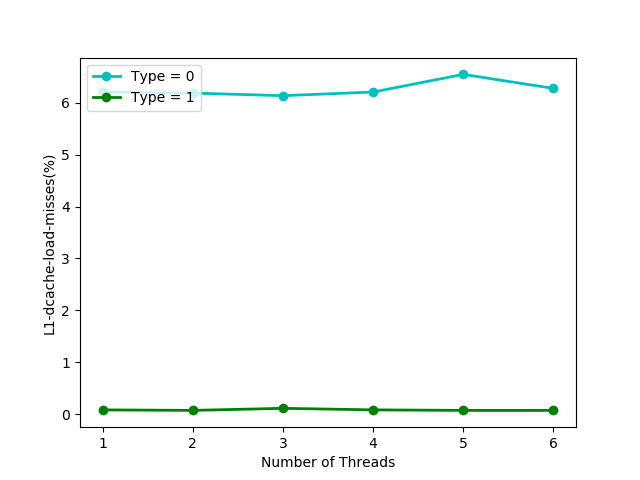
\includegraphics[width=10cm]{cache-analysis-perf.png}
    \caption{Cache Comparision: perf}
\end{figure}


\section{valgrind}
Valgrind is also a detailed profiler taht provides not only cache analysing tools but also tools to analyse the runtime of different parts of code and compare them. It also provides features using which we can check memory leaks inside code. \\
I cheked for any memory leak, there wasn't any. Thereafter I used cachegrind tool of valgrind to study the cache behaviour of modified code that I got through optimisations done using perf.\\

I used the command: 
\begin{center}
    'valgrind --tool=cachegrind ./classify rfile dfile 1009072 4 3'
\end{center}
\textsc{NOTE: } One thing that I noticed while using valgrind is that, out of all 3 profilers this took the highest time to run the code. Moreover other 2 did not had any resonable overhead on time but valgrind took a lot more time than simply running the same code (without any profiler).
\subsection{Original Code: }
Following are the results:- \\
\begin{figure}[H]
    \centering
    \includegraphics[width=12cm]{valgrind0.png}
    \caption{Original Code: valgrind}
\end{figure}
\subsection{Modified Code: }
Following are the results:- \\
\begin{figure}[H]
    \centering
    \includegraphics[width=12cm]{valgrind1.png}
    \caption{Modified Code: valgrind}
\end{figure}

\subsection{Comparision: }
I wrote a python script to run original and modified code on varying number of threads and plotted the graph of cache misses. Here are the results for D1 cache misses noted from valgrind:- \\
\begin{figure}[H]
    \centering
    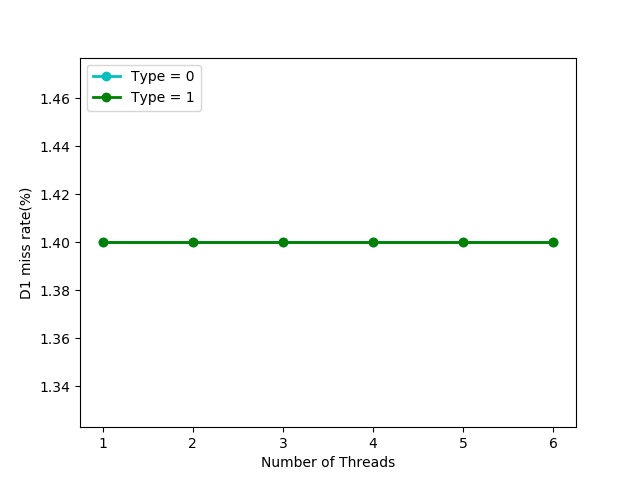
\includegraphics[width=10cm]{cache-analysis-valgrind.png}
    \caption{Cache Comparision: valgrind}
\end{figure}

\section{gprof}
This is a very old profiler (in use since 80's) and provides many featues to analyse the code on the basis of make parameters, like function taking most amount of time, function call graph etc. But one drawback of this profiler is that it only analyse the main thread of process. Hence I was not able to do any optimisation using the results of this profiler.  
\subsection{Original Code: }

\begin{enumerate}
    \item \textbf{gprof --flat-profile classify}\\
    \begin{figure}[H]
        \centering
        \includegraphics[width=12cm]{gprof0.png}
        \caption{Original Code: gprof --flat-profile}
    \end{figure}

    \item \textbf{gprof --graph classify}\\
    \begin{figure}[H]
        \centering
        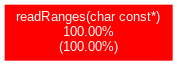
\includegraphics[width=12cm]{gprofc0.png}
        \caption{Original Code: gprof --graph}
    \end{figure}
\end{enumerate}




\subsection{Modified Code: }
\begin{enumerate}
    \item \textbf{gprof --flat-profile classify}\\
    \begin{figure}[H]
        \centering
        \includegraphics[width=12cm]{gprof1.png}
        \caption{Modified Code: gprof --flat-profile}
    \end{figure}

    \item \textbf{gprof --graph classify}\\
    \begin{figure}[H]
        \centering
        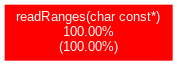
\includegraphics[width=12cm]{gprofc1.png}
        \caption{Modified Code: gprof --graph}
    \end{figure}
\end{enumerate}


\subsection{Time Comparision: }
Finally when all analysis was done I plotted the number of threads vs runtime graph for original and modified code. Here are the results:- \\
\begin{figure}[H]
    \centering
    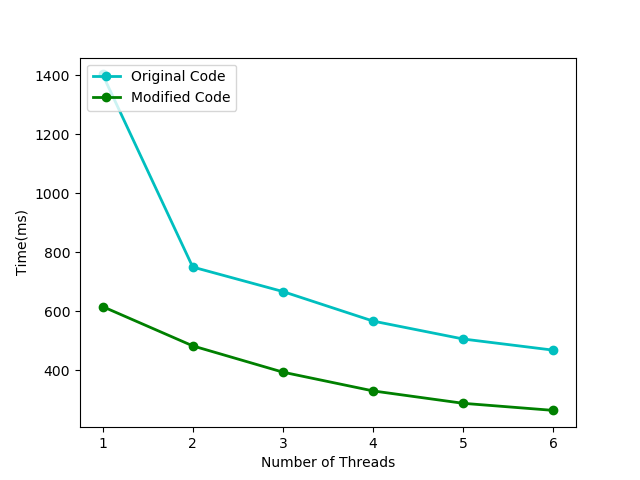
\includegraphics[width=10cm]{time-analysis.png}
    \caption{Time Comparision: local}
\end{figure}

I also plotted the same graph by running the plotting script on palasi VM to double check. Here are the results:- 
\begin{figure}[H]
    \centering
    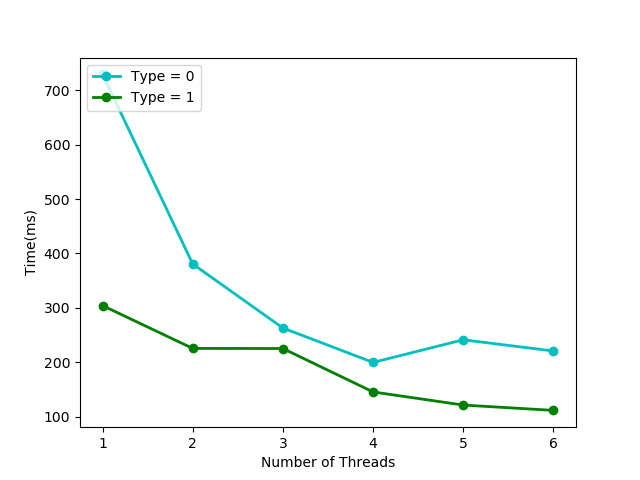
\includegraphics[width=10cm]{time-analysis-vm.png}
    \caption{Time Comparision: VM}
\end{figure}

\end{document}
